\documentclass[a4paper,11pt, twocolumn]{article}
\usepackage[margin=0.8in]{geometry}
\usepackage{xcolor}
\usepackage{graphicx} %package to manage images
\graphicspath{ {./images/} }
\usepackage{tabularx}
\usepackage{float}
\usepackage{multirow}
\usepackage[fleqn]{mathtools}
\usepackage{amsmath}
\usepackage{amssymb}

\title{1.4.3 Boolean Algebra}
\author{Revision sheet}
\date{}

\usepackage{fancyhdr}
\pagestyle{fancy}
\fancyhead{} % clear all header fields
\renewcommand{\headrulewidth}{0pt} % no line in header area
\fancyfoot{} % clear all footer fields
\renewcommand{\footrulewidth}{0.4pt}
\fancyfoot[C]{\thepage} % page number in centre of the page
\fancyfoot[R]{\footnotesize Thomas Boxall \\ Images from WJEC Electronics E-Book \& CS Textbook } % right hand footer has author name on top line and images reference on bottom line
\fancyfoot[L]{\footnotesize 1.4.3 Boolean Algebra \\ Revision sheet} % left hand footer has title of document on top line and 'Revision Sheet' on bottom line


\begin{document}

\maketitle
\thispagestyle{fancy}

% CONTENTS OF THE REVISION SHEET HERE
\section{Boolean Algebra}
In the following sections, the Boolean algebra have been expressed using the standard Electronics notation. This will be accepted in the exams however questions will be given using the following OCR notation.
\subsection{OCR Boolean Algebra Notation}
\begin{table}[H]
    \centering
    \begin{tabular}{c | c c }
        Operator & OCR & Electronics \\
        \hline
        AND & $A \bigwedge B$ & $A \cdot B$ \\
        OR  & $A \bigvee B$ & $A + B$ \\
        NOT & $\neg A$ & $\overline{A}$ \\
        XOR & $A \veebar B$ & $A \oplus B$
    \end{tabular}
    \caption{Comparison of OCR and electronics Boolean algebra operators}
    \label{tab:ocrVsEle}
\end{table}
\noindent For expressions where the components are only shown in Electronics notation below, they can be constructed from multiple of the OCR symbols shown above.

\section{Logic Gates and Truth Tables}
For the most part, logic gates can have multiple inputs and one output. Pictured here are the smallest arrangement they come in. In real life, logic gates come in chips, generally bundled into sets of 4 or 6 in one chip.
\subsection{AND Gate}
This only outputs when all inputs are logic high.
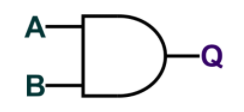
\includegraphics[width=0.2\textwidth]{andGate.PNG}
\begin{table}[H]
    \centering
    \begin{tabularx}{0.127\textwidth}{c|c|c}
    B & A & Q \\
    \hline
    0 & 0 & 0 \\
    0 & 1 & 0 \\
    1 & 0 & 0 \\
    1 & 1 & 1
    \end{tabularx}
    \caption{Truth Table for AND Gate}
\end{table}
Boolean Expression: $Q=A \cdot B$
\subsection{OR Gate}
This outputs 1 when either or both are logic high.
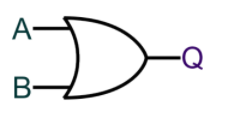
\includegraphics[width=0.2\textwidth]{orGate.PNG}
\begin{table}[H]
    \centering
    \begin{tabularx}{0.127\textwidth}{c|c|c}
    B & A & Q \\
    \hline
    0 & 0 & 0 \\
    0 & 1 & 1 \\
    1 & 0 & 1 \\
    1 & 1 & 1
    \end{tabularx}
    \caption{Truth Table for OR Gate}
\end{table}
Boolean Expression: $Q=A+B$
\subsection{NOT Gate}
This is a single input gate. It inverts the signal in.\\
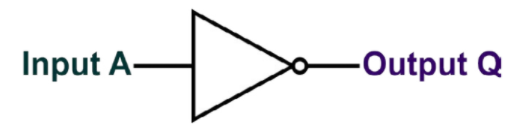
\includegraphics[width=0.2\textwidth]{notGate.PNG}
\begin{table}[H]
    \centering
    \begin{tabularx}{0.085\textwidth}{c|c}
    A & Q \\
    \hline
    0 & 1 \\
    1 & 0 \\
    \end{tabularx}
    \caption{Truth Table for NOT Gate}
\end{table}
Boolean Expression: $Q=\overline{A}$
\subsection{XOR Gate}
This outputs only when input A or B is logic high - eXclusiveOR.\\
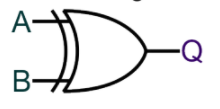
\includegraphics[width=0.2\textwidth]{xorGate.PNG}\\
\begin{table}[H]
    \centering
    \begin{tabularx}{0.127\textwidth}{c|c|c}
    B & A & Q \\
    \hline
    0 & 0 & 0 \\
    0 & 1 & 1 \\
    1 & 0 & 1 \\
    1 & 1 & 0
    \end{tabularx}
    \caption{Truth Table for XOR Gate}
\end{table}
Boolean Expression: $Q = A \oplus B $
\subsection{NAND Gate}
This is the same as an AND gate, except it inverts the output.\\
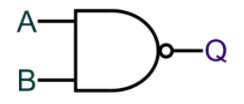
\includegraphics[width=0.2\textwidth]{nandGate.PNG}\\
\begin{table}[H]
    \centering
    \begin{tabularx}{0.127\textwidth}{c|c|c}
    B & A & Q \\
    \hline
    0 & 0 & 1 \\
    0 & 1 & 1 \\
    1 & 0 & 1 \\
    1 & 1 & 0
    \end{tabularx}
    \caption{Truth Table for NAND Gate}
\end{table}
Boolean Expression: $Q = \overline{A \cdot B}$
\subsection{NOR Gate}
This only outputs logic high if both inputs are logic 0 - NotOR. This makes it useful for checking if something is 0.\\
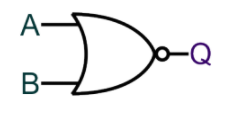
\includegraphics[width=0.2\textwidth]{norGate.PNG}\\
\begin{table}[H]
    \centering
    \begin{tabularx}{0.127\textwidth}{c|c|c}
    B & A & Q \\
    \hline
    0 & 0 & 1 \\
    0 & 1 & 0 \\
    1 & 0 & 0 \\
    1 & 1 & 0
    \end{tabularx}
    \caption{Truth Table for NOR Gate}
\end{table}
Boolean Expression: $Q=\overline{A + B}$
\subsection{XNOR Gate}
This outputs if all inputs are logic 0 or if all inputs are logic 1 - eXclusiveNotOR. This is useful for checking if the inputs are the same.\\
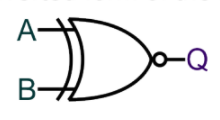
\includegraphics[width=0.2\textwidth]{xnorGate.PNG}\\
\begin{table}[H]
    \centering
    \begin{tabularx}{0.127\textwidth}{c|c|c}
    B & A & Q \\
    \hline
    0 & 0 & 1 \\
    0 & 1 & 0 \\
    1 & 0 & 0 \\
    1 & 1 & 1
    \end{tabularx}
    \caption{Truth Table for XNOR Gate}
\end{table}
Boolean Expression: $Q=\overline{A \oplus B}$

\section{Manually Simplifying Boolean Algebra}
\subsection{Boolean Identities}
$A\oplus B = A \cdot \overline{B} + \overline{A} \cdot B$\\
$\overline{A\oplus B} = A\cdot B + \overline{A} \cdot \overline{B}$
\subsection{Single Variable Rules}
\begin{align*}
    A \cdot 0 &= 0\\
    A \cdot 1 &= A\\
    A \cdot A &= A\\
    A \cdot \overline{A} &= 0\\
    A + 0 &= A\\
    A + 1 &= 1\\
    A + A &= A\\
    A + \overline{A} &= 1
\end{align*}
\subsection{Rules}
\subsubsection{Commutative}
The order doesn't matter.\\
\begin{align*}
    A \cdot B &= B \cdot A\\
    A + B &= B + A
\end{align*}
\subsubsection{Associative}
Some can be re-grouped to make simplification easier.\\
\begin{align*}
    A+(B+C) &= (A+B)+C\\
    &= A+B+C\\ \\
    A\cdot (B\cdot C) &= (A\cdot B) \cdot C \\
    &= A \cdot B \cdot C
\end{align*}
\subsubsection{Distributive}
\begin{align*}
    A\cdot B + A\cdot C &= A(B+C)\\
    C\cdot (B\cdot A + D) &= C\cdot B\cdot A + C \cdot D\\
    (A\cdot B)\cdot (C\cdot D) &= A\cdot C + A\cdot D + \\
    & \ \ \ \ B\cdot C + B\cdot D\\
    A+(B\cdot C) &= (A+B)\cdot (A+C)
\end{align*}
\subsubsection{Absorption / Redundancy}
\begin{align*}
    A+A \cdot B &= A\\
    A+\overline{A} \cdot B &= A+B
\end{align*}
\subsubsection{Double Inversion}
\begin{align*}
    \overline{\overline{A}} &=A
\end{align*}
\subsection{deMorgan's Theorem}
\textit{Break the bar, change the sign}.
\begin{align*}
    \overline{A\cdot B} &= \overline{A} + \overline{B}\\
    \overline{A+B} &= \overline{A}\cdot \overline{B}
\end{align*}

\section{Karnaugh Maps}
Karnaugh maps can be used to simplify boolean algebra expressions. In their simplest form, they have a grid of two across and two down. This is the size which would be needed to simplify a boolean expression for a single logic gate.\\
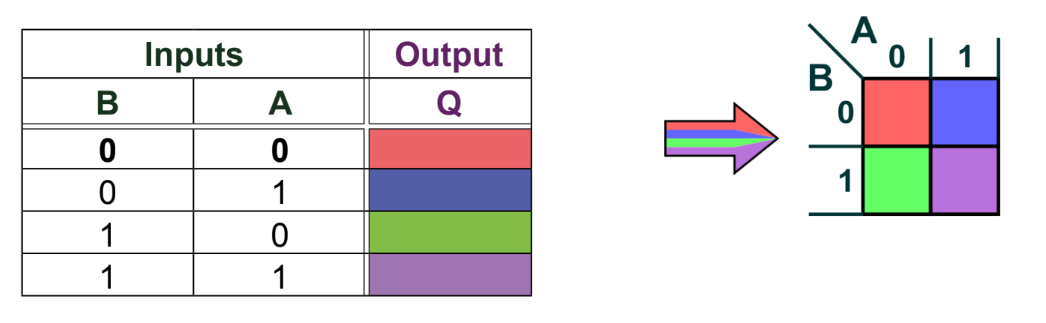
\includegraphics[width=0.45\textwidth]{kMaps1.PNG}\\
\subsection{Simplification using a Karnaugh Map}
Karnaugh maps allow us to simplify boolean expressions graphically. This works by identifying groups of 2, 4 or 8 neighbouring cells containing logic 1 (these can also wrap around the edge of the table); finding the term common to each groups then combining the terms together using the OR operator. Every cell containing logic 1 must be included in at least one group.
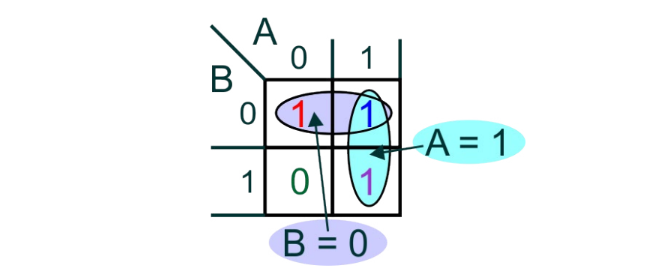
\includegraphics[width=0.45\textwidth]{kMaps2.PNG}\\
In the example above, the top right cell is in two groups, this is okay as long as each group as at least one of the cells in the group is only in one group. The cells in the blue group are in the A=1 column, this means the term common to them is $A$. The cells in the purple group are in the B=0 row, this means the term common to them is $\overline{B}$. Combining the blue and purple group gives us $Q=\overline{B} + A$.
\subsection{Bigger Karnaugh Maps}
Karnaugh maps can have many more inputs. Shown below are three-input and four-input Karnaugh maps.\\
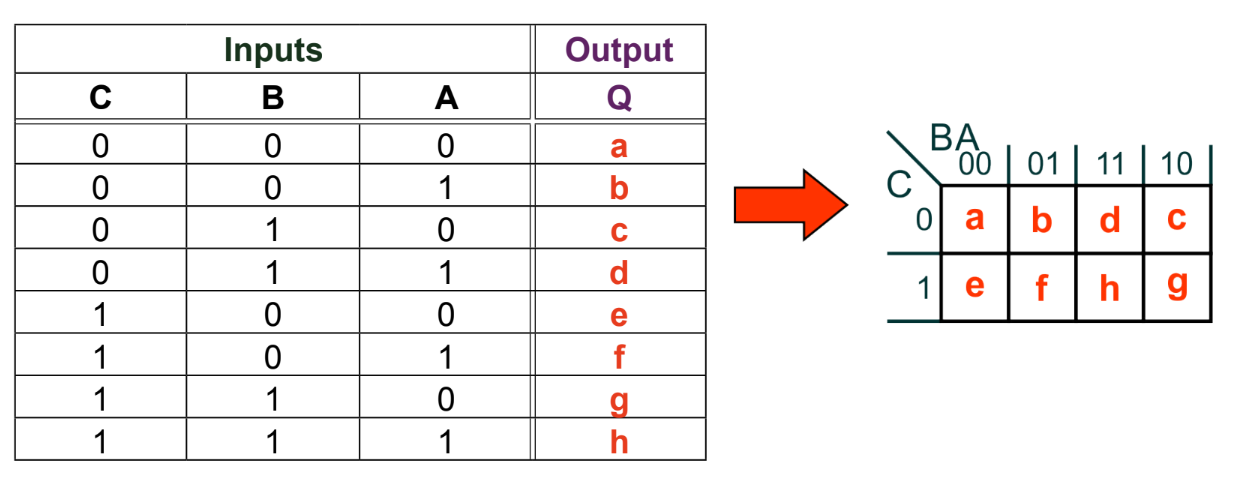
\includegraphics[width=0.45\textwidth]{kMaps CBA inp.PNG}\\
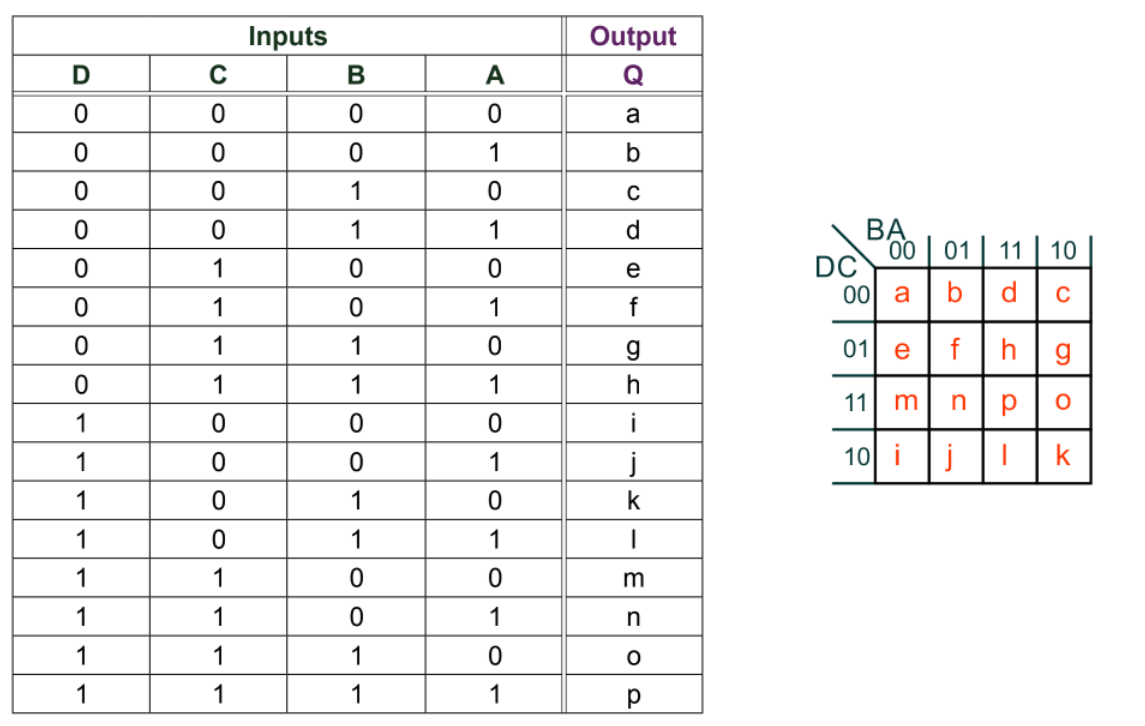
\includegraphics[width=0.45\textwidth]{kMaps DCBA inp.PNG}\\

\section{D Flip-Flops}
A \textit{D-type flip-flop} is a positive edge-triggered flip-flop (this means that the output will only change when the clock is at a rising edge). A D-type flip-flop has four connections, two input and two output. The inputs are $D$ and $CLK$, which stands for clock, and the outputs are $Q$ and $\overline{Q}$, which is inverted $Q$.\\
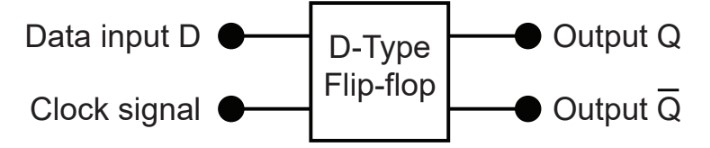
\includegraphics[width=0.45\textwidth]{d-flop.jpg}\\
Whenever the clock pulse is recieved into the flip flop, whatever the D value is will be moved to the output. This is the same for when D is logic high or logic low. The relationship between these three ports can be shown on a timing diagram (shown below).\\
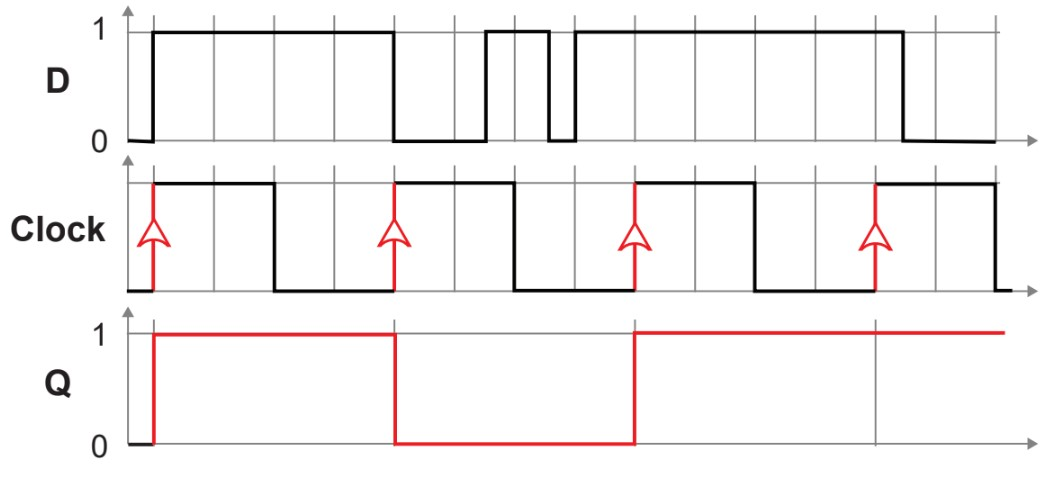
\includegraphics[width=0.45\textwidth]{d-flopTiming.jpg}\\
D flip-flops can be used as register memory locations as they will only store the data for one clock cycle. 

\section{Adders}
With the right combination of logic gates, it is possible to output the result of a binary addition or subtraction including the value of any carry bit as a second output. There are two types of adders.
\subsection{Half-Adder}
This can take an input of two bits and give a two-bit output.\\
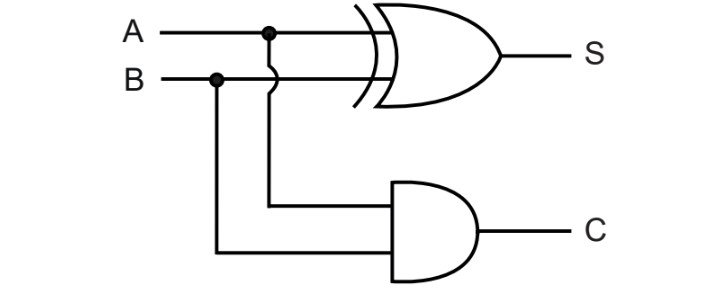
\includegraphics[width=0.45\textwidth]{halfAdder.jpg}\\
A half adder has the following truth table.\\
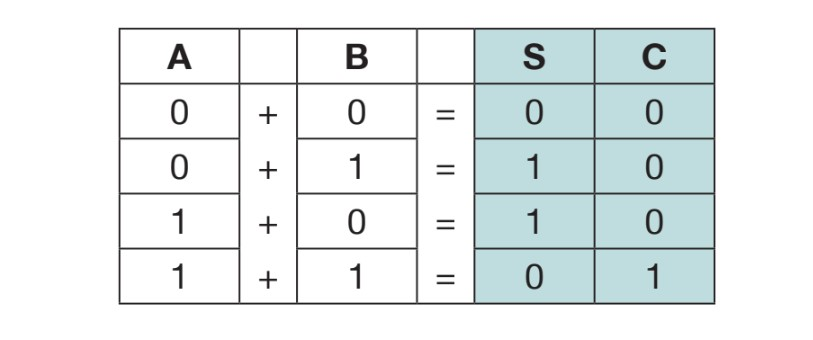
\includegraphics[width=0.45\textwidth]{halfAdderTable.jpg}\\
\subsection{Full-Adder}
A full adder combines two half adders together which allows three bits to be added together (A, B and a carry bit C). \\
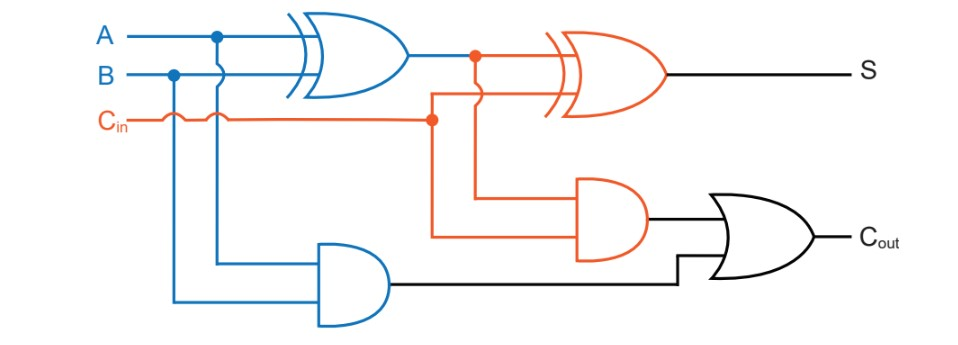
\includegraphics[width=0.45\textwidth]{fullAdder.jpg}\\
A full adder has the following truth table.\\
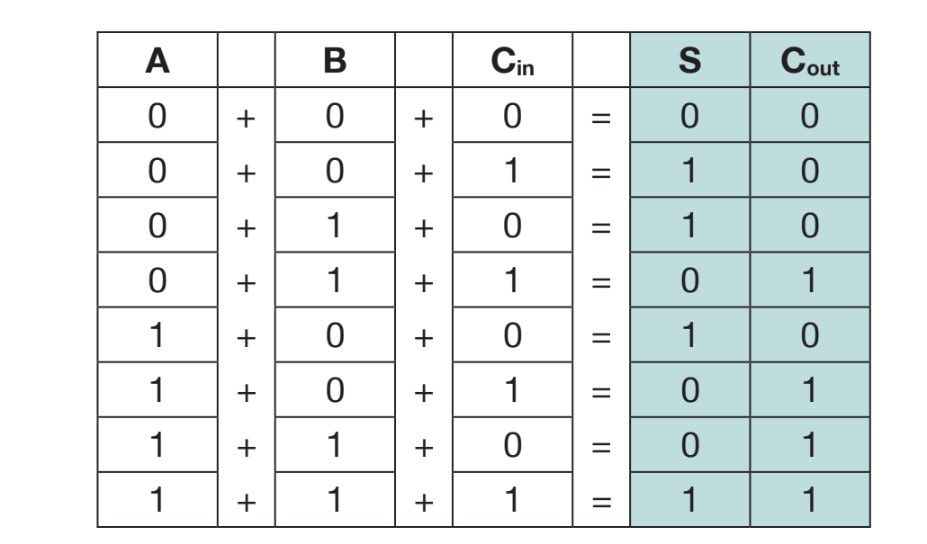
\includegraphics[width=0.45\textwidth]{fullAdderTable.jpg}
\subsection{Combining Adders}
To add numbers which are bigger than one bit together, you will need to combine multiple full adders together. They can be done so as follows.\\
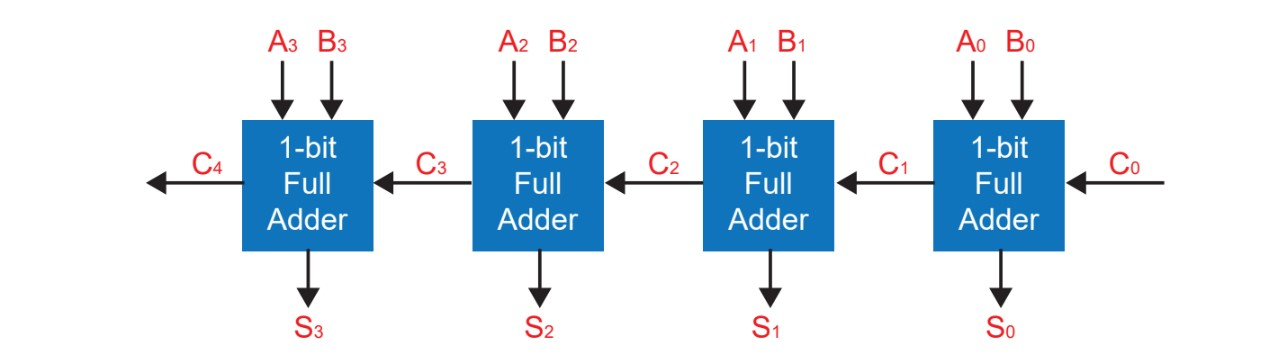
\includegraphics[width=0.45\textwidth]{manyAdders.jpg}




\end{document}

t (a) Define problems using Boolean logic. See appendix 5d.
t(b) Manipulate Boolean expressions, including the use of Karnaugh maps to simplify Boolean expressions.
t(c) Use the following rules to derive or simplify statements in Boolean algebra: De Morgan’s Laws, distribution, association, commutation, double negation.
t(d) Using logic gate diagrams and truth tables. See appendix 5d.
(e) The logic associated with D type flip flops, half and full adders.